%%%%%%%%%%%%%%%%%%%%%%%%%%%%%%%%%%%%%%%%%%%%%%%%%%%%%%%%%%
%%
%% MARK: Title
%%
%%%%%%%%%%%%%%%%%%%%%%%%%%%%%%%%%%%%%%%%%%%%%%%%%%%%%%%%%%

\chapter*{\S B23. Diffeomorphisms of $\Geod(\Torus^2)$}
\setcounter{footnote}{0}

%%%%%%%%%%%%%%%%%%%%%%%%%%%%%%%%%%%%%%%%%%%%%%%%%%%%%%%%%%
%%
%% MARK: Abstract
%%
%%%%%%%%%%%%%%%%%%%%%%%%%%%%%%%%%%%%%%%%%%%%%%%%%%%%%%%%%%

\begin{abstract}
  In this note we describe the group of diffeomorphisms of the space of geodesic trajectories of the $2$-torus.
\end{abstract}

%%%%%%%%%%%%%%%%%%%%%%%%%%%%%%%%%%%%%%%%%%%%%%%%%%%%%%%%%%
%%
%% MARK: Geodesic Trajectories of the $2$-Torus
%%
%%%%%%%%%%%%%%%%%%%%%%%%%%%%%%%%%%%%%%%%%%%%%%%%%%%%%%%%%%
\section{Geodesic trajectories of the $2$-torus}

We consider the space of geodesic trajectories of the $2$-torus $\Torus^2 = \RR^2/\ZZ^2$,
see §B20: ``The geodesics of the $2$-torus'' in these notes.
They are the projections of the affine lines in $\RR^2$ by the projection $\Class : \RR^2 \to \Torus^2$:
$$%
  \Class : (x,y) \mapsto \big(e^{2i\pi x}, e^{2i\pi y}\big).
  $$%

\begin{Article}{The geodesics of $\RR^2$}{}
  The set of (oriented) affine lines in $\RR^2$ is diffeomorphic to the tangent bundle of the circle $\Sph^1$.
  That is:
  $$%
    \Geod(\RR^2) \simeq \TgtBundle{\Sph^1} = \big\{ (u,r) \in \Sph^1 \times \RR^2 \mid u \cdot r = 0 \big\}.
    $$%
  With every pair $(u,r)$ is associated the line
  $$%
    \Delta(u,r) = \{r + tu\}_{t \in \RR}.
    $$%
  This space is also equivalent to $\Sph^1 \times \RR$,
  thanks to the mapping
  $$%
    (u,r) \mapsto (u, \rho = u \cdot \J r),
    \quad \text{with} \quad
    \J = \Vector{0 & -1 \\ 1 & 0}.
    $$%
  The centered dot denotes the scalar product.
\end{Article}

\begin{figure}[th]
  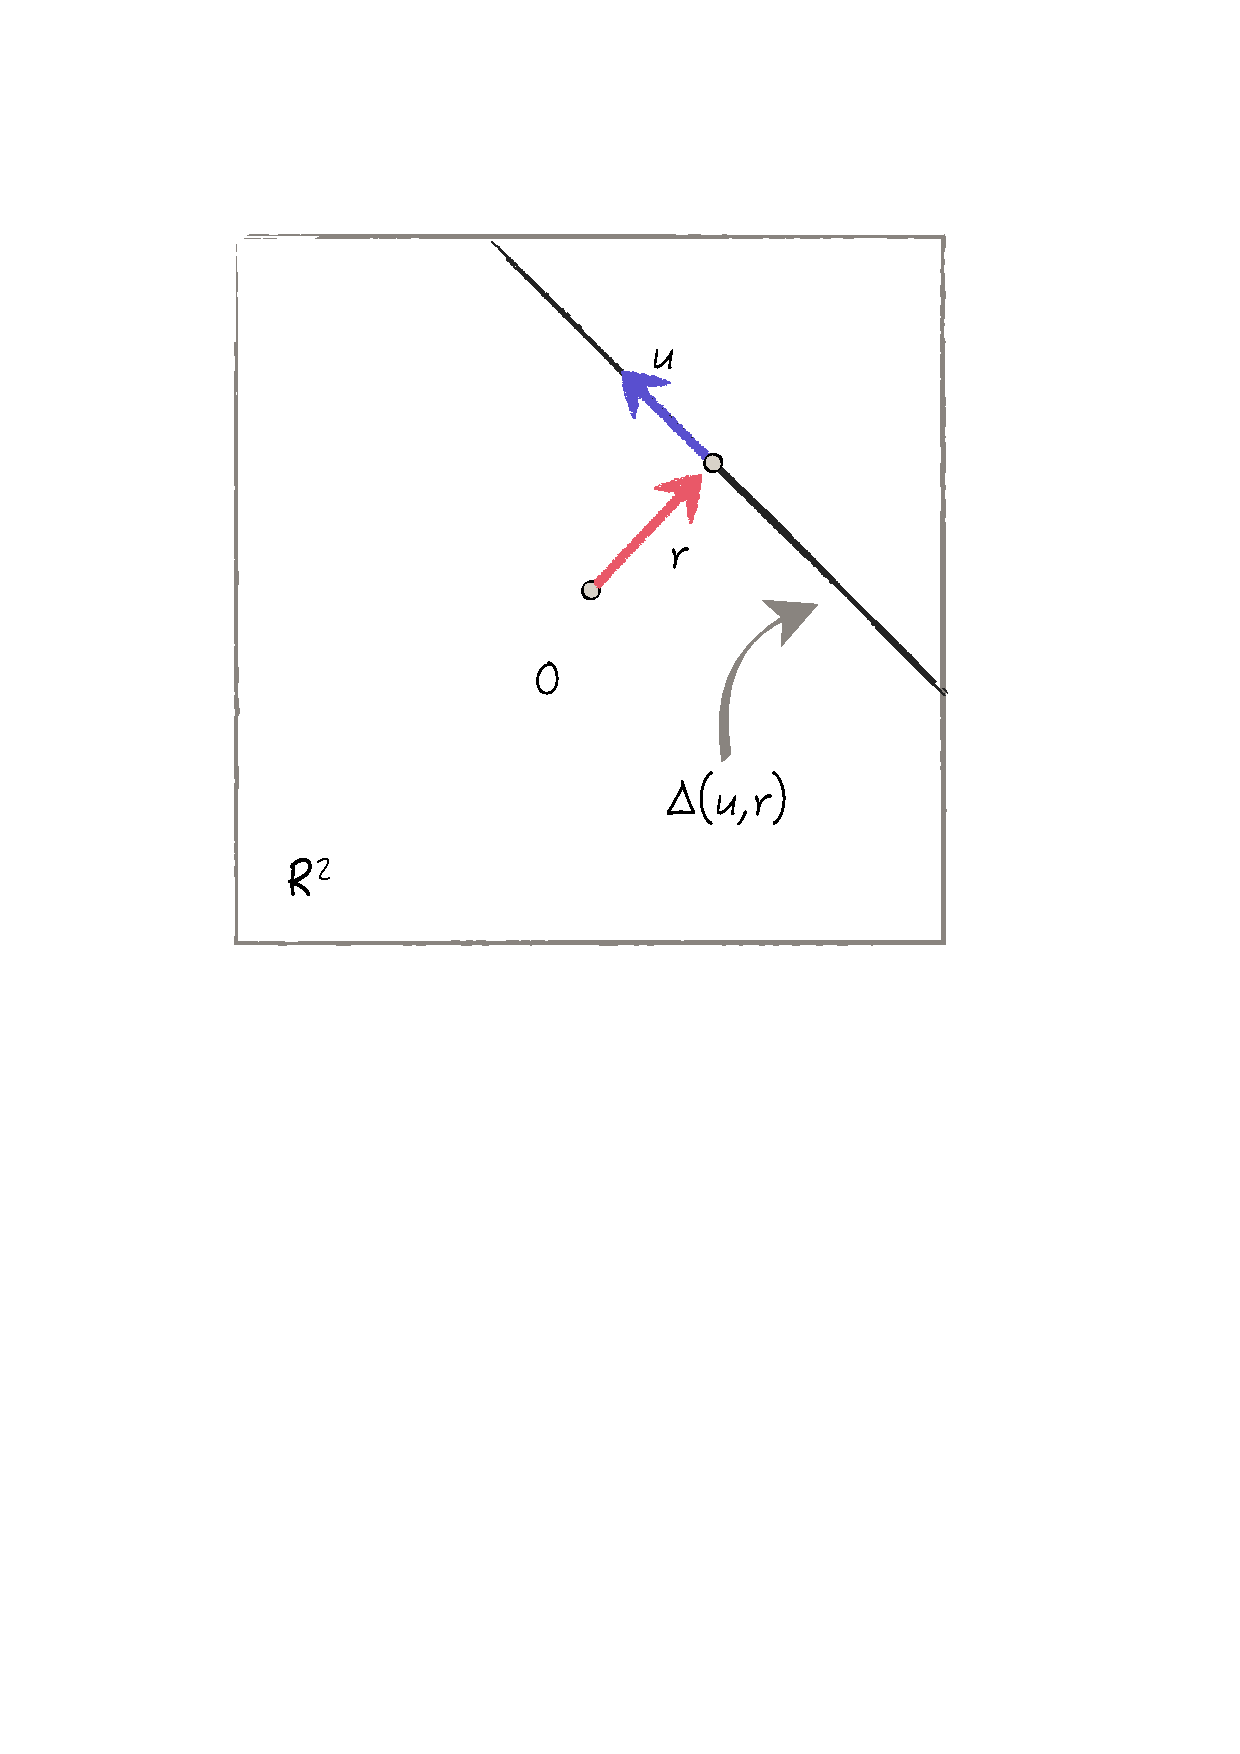
\includegraphics[width=.5\textwidth]{Figures/Geod-R2.pdf}
  \vspace{-.25\baselineskip}
  \caption{The geodesic trajectories of the plane.}
  \label{Geod-R2.pdf}
\end{figure}

\begin{proof}
  Contained in Figure \ref{Geod-R2.pdf}.
\end{proof}

\begin{Article}{The geodesics of $\Torus^2$}{}
  The set of (oriented) affine lines in $\Torus^2$ is diffeomorphic to the quotient space
  $$%
    \Geod(\Torus^2) \simeq (\Sph^1 \times \RR) / \ZZ^2,
    $$%
  with the $\ZZ^2$-action defined by
  $$%
    \underline{k}(u,\rho) = (u, \rho + u \cdot k)
    \quad \text{for all} \quad
    k = (m,n) \in \ZZ^2.
    $$%
\end{Article}

Let $u = (\cos(\theta), \sin(\theta))$,
the action of $\ZZ^2$ on $\Sph^1 \times \RR$ becomes
$$%
  \underline{(m,n)}(u,\rho) = (u, \rho + m \cos(\theta) + n \sin(\theta)).
  $$%
We denote
$$%
  \Class(u,\rho) \equiv (u, \Class_u(\rho)) = \big(u, \{\rho + k \cdot u \mid k \in \ZZ^2 \}\big),
  $$%
and
$$%
  \Proj_1 : (u, \Class_u(\rho)) \mapsto u,
  $$%
the projection of $\Geod(\Torus^2)$ onto $\Sph^1$.

\begin{Article}{The projection onto the circle}{}
  The fiber of the projection $\Proj_1$ is the torus
  $$%
    \Torus_u = \RR/[\ZZ \cos(\theta) + \ZZ \sin(\theta)].
    $$%
  The torus $\Torus_u$ is irrational when $\cos(\theta)$ and $\sin(\theta)$ are independent over $\QQ$, and rational,
  diffeomorphic to a circle $\RR/a\ZZ$,
  otherwise.
  
  It has a group structure:
  $$%
    \Class_u(\rho) + \Class_u(\rho') = \Class_u(\rho + \rho').
    $$%
  The projection $\Proj_1$ has a global section:
  $$%
    \sigma \in \Cinfty(\Sph^1, \Geod(\Torus^2)), \quad \sigma : u \mapsto \Class_u(0).
    $$%
  These are the geodesic trajectories passing through $0 \in \RR^2$.
\end{Article}

%%%%%%%%%%%%%%%%%%%%%%%%%%%%%%%%%%%%%%%%%%%%%%%%%%%%%%%%%%
%%
%% MARK: Diffeomorphisms of $\Geod(T^2)$
%%
%%%%%%%%%%%%%%%%%%%%%%%%%%%%%%%%%%%%%%%%%%%%%%%%%%%%%%%%%%
\section{Diffeomorphisms of $\Geod(T^2)$}

The diffeology of $\Geod(\Torus^2)$ is defined as the quotient diffeology of the manifold $\Sph^1 \times \RR$ by $\ZZ^2$,
and then
$$%
  \Geod(\Torus^2) \simeq \RR^2/\ZZ^3,
  $$%
where $(\ell,m,n) \in \ZZ^3$ acts on $\RR^2$ by:
$$%
  (\ell, m, n)_{\RR^2}(\theta,\rho) = (\theta + 2\pi\ell, \rho + m \cos(\theta) + n \sin(\theta)).
  $$%

\begin{Article}{Proposition 1}{}
  Let $f \in \Diff(\Geod(\Torus^2))$,
  then there exists $M \in \GL(2,\ZZ)$ such that
  $$%
    \Proj_1 \circ f = \underline M \circ \Proj_1,
    $$%
  where $\GL(2,\ZZ)$ acts on $\Sph^1$ by
  $$%
    \underline M (u) =  u'
    \quad \Leftrightarrow \quad u' = \frac{M u}{\|M u\|}.
    $$%
  Let us call $\Psi$ the homomorphism
  $$%
    \Psi : \Diff(\Geod(\Torus^2)) \to \GL(2,\ZZ)
    \quad \text{with} \quad
    \Psi(f) = M.
    $$%
  We have a short exact sequence of homomorphisms:
  $$%
    0  \to  \ker(\Psi) \to \Diff(\Geod(\Torus^2)) \to \GL(2,\ZZ) \to 0.
    $$%
\end{Article}

\begin{proof}
  Let $f \in \Diff(\Geod(\Torus^2))$.
  The plot $f \circ \Class \circ \Class_1$ has a local smooth lifting $\Phi$,
  that is,
  $$%
    f \circ \Class \circ \Class_1 =_\loc \Class \circ \Class_1 \circ \Phi.
    $$%
  Precisely,
  if
  $$%
    \Phi(\theta,\rho) = (\theta',\rho')
    $$%
  then,
  for all $(\theta,\rho) \in \RR^2$ and all $(\ell,m,n) \in \ZZ^3$ there exists $(\ell',m',n') \in \ZZ^3$ such that:
  $$%
    \Phi(\theta + 2\pi\ell, \rho + m \cos(\theta) + n \sin(\theta)) = (\theta' + 2\pi\ell', \rho' + m' \cos(\theta') + n' \sin(\theta')).
    $$%
  Denoting
  $$%
    \pphi\big(\Class_1(\theta,\rho)\big) = \Class_1\big(\Phi(\theta, \rho)\big)
    \quad \text{with} \quad
    \Class_1(\theta, \rho) = \big(e^{i\theta}, \rho\big),
    $$%
  we have
  $$%
    \Class_1 \circ \Phi =_\loc \pphi \circ \Class_1,
    $$%
  and therefore
  $$%
    \Class \circ \pphi =_\loc f \circ \Class.
    $$%
  
  \begin{center}
    \begin{tikzcd}[column sep=large, row sep=large, every label/.append style = {font = \small}]
      \RR \times \RR  \arrow[r, dashed, "\Phi"] \arrow[d, swap, "\Class_1"]  & \RR \times \RR \arrow[d, "\Class_1"]   \\
      \Sph^1 \times \RR  \arrow[r, dashed, "\pphi"] \arrow[d, swap, "\Class"]  & \Sph^1 \times \RR \arrow[d, "\Class"]   \\
      \Geod(\Torus^2) \arrow[r, swap, "f"] & \Geod(\Torus^2)
    \end{tikzcd}
  \end{center}
  
  Let $(u,\rho) \in \Sph^1 \times \RR$:
  $$%
    \pphi(u,\rho) = (u',\rho')
    \quad \text{with} \quad
    u' = \cU(u,\rho)
    \quad \text{and} \quad
    \rho' = \cR(u,\rho).
    $$%
  For all $k \in \ZZ^2$,
  there exists $k' \in \ZZ^2$,
  depending a priori on $k, u, \rho$, such that:
  $$%
    \pphi\big(\underline{k}(u,\rho)\big) = \underline{k'}\big(\pphi(u,\rho)\big).
    $$%
  We denote by $\underline{k}$ the action of $k \in \ZZ^2$.
  Thus,
  \begin{align*}
    \pphi(u, \rho + u \cdot k) & = \underline{k'}(u',\rho') \\
    \big(\cU(u,\rho + k \cdot u), \cR(u,\rho + k \cdot u)\big) & = (u', \rho' + u' \cdot k') \\
    \big(\cU(u,\rho + k \cdot u), \cR(u,\rho + k \cdot u)\big) & = \big(\cU(u,\rho), \cR(u,\rho) + \cU(u,\rho) \cdot k').
  \end{align*}
  We obtain:
  $$%
    \left\{
    \begin{aligned}
    \cU(u,\rho + k \cdot u) & =  \cU(u,\rho) \hfill & (\diamondsuit) \\
    \cR(u,\rho + k \cdot u) & =  \cR(u,\rho) + \cU(u,\rho) \cdot k' & (\heartsuit)
    \end{aligned}
    \right.
    $$%
  The first identity $(\diamondsuit)$ gives
  $$%
    \cU(u,\rho) = \cU(u, \rho + m \cos(\theta) + n \sin(\theta)),
    $$%
  where $u = (\cos(\theta), \sin(\theta))$ and for all $m,n \in \ZZ$.
  Then,
  for all irrational $u$,
  by density of $\{m \cos(\theta) + n \sin(\theta) \mid m,n \in \ZZ\}$ in $\RR$,
  we have:
  $$%
    \cU(u,\rho) = \cU(u,0).
    $$%
  Then,
  because the set of irrational $u$ is dense in $\Sph^1$:
  $$%
    \text{For all } u \in \Sph^1, \quad u' = \cU(u)
    $$%
  is independent of $\rho$.
  Thus,
  the map $\pphi$ can be written as
  $$%
    \pphi : (u,\rho) \mapsto (u' = \cU(u), \rho' = \cR(u,\rho)).
    $$%
  The map $f$ then becomes
  $$%
    f(u, \Class_u(\rho)) = \big(u' = \cU(u), \Class_{u'}(\cR(u,\rho))\big).
    $$%
  Thus,
  $f$ sends the fiber $\Torus_u$ to $\Torus_{u'}$,
  and the restriction of $f$ to $\Torus_u$ is given by
  $$%
    f_u : \Class_u(\rho) \mapsto \Class_{u'}(\rho')
    \quad \text{with} \quad
    \rho' = \cR(u,\rho).
    $$%
  But since $f$ is a diffeomorphism,
  its restriction to $\Torus_u$ is a diffeomorphism:
  $$%
    f_u = f \restriction \Torus_u \in \Diff(\Torus_u, \Torus_{u'}).
    $$%
  There exists then a map $F : \Sph^1 \to \Sph^1$ such that $u' = F(u)$ and the following diagram commutes:
  
  \begin{center}
    \begin{tikzcd}[column sep=large, row sep=large, every label/.append style = {font = \small}]
      \Geod(\Torus^2) \arrow[d, swap, "\Proj_1"] \arrow[r, "f"] & \Geod(\Torus^2) \arrow[d, "\Proj_1"] \\
      \Sph^1  \arrow[r, swap, "F"]  & \Sph^1
    \end{tikzcd}
  \end{center}
  
  The map $F$ is a diffeomorphism because $f$ is a diffeomorphism and the projection $\Proj_1$ is a subduction.
  Thus,
  $f$ is an automorphism of the projection $\Proj_1$:
  $$%
    [f \mapsto F] \in \Hom^\infty\big(\Diff(\Geod(\Torus^2)), \Diff(\Sph^1)\big).
    $$%
  On the other hand,
  we know \cite{DI83} that $\Torus_u$ and $\Torus_{u'}$ are diffeomorphic if and only if:
  $$%
    u' = F(u) \quad \Rightarrow \quad \exists M \in \GL(2,\ZZ), \ M u = \lambda u' \text{ for some } \lambda > 0.
    $$%
  Said differently,
  $$%
    \exists M \in \GL(2,\ZZ), \ \RR u' = M(\RR u).
    $$%
  A priori $M$ depends on $u$.
  Consider the circle $\Sph^1$ as the set of directions in $\RR^2$,
  that is,
  $$%
    \Sph^1 = [\RR^2 \setminus \{0\}] / ]0,\infty[
    \quad \text{with} \quad
    \Vector{x \\ y} \sim \lambda \Vector{x \\ y}
    \quad \text{for all} \quad
    \lambda \in ]0,\infty[.
    $$%
  The map $F$ has a lifting (at least locally) to $\RR^2 \setminus \{0\}$.
  Call it $\tilde F$:
  
  $$%
    \begin{tikzcd}[column sep=large, row sep=large, every label/.append style = {font = \small}]
    \RR^2 \setminus \{0\} \arrow[d, swap, "\Class"] \arrow[r, dashed, "\tilde F"] & \RR^2 \setminus \{0\} \arrow[d, "\Class"] \\
    \Sph^1  \arrow[r, swap, "F"]  & \Sph^1
    \end{tikzcd}
    \qquad \Class \circ \tilde F =_\loc F \circ \Class.
    $$%
  
  Thus,
  for all $u \in \Sph^1$,
  for all $v = (x,y) \in \RR u$,
  we have
  $$%
    \tilde F \Vector{x \\ y} = \Vector{a_u & b_u \\ c_u & d_u} \Vector{x \\ y}
    \quad \text{with} \quad
    M_u = \Vector{a_u & b_u \\ c_u & d_u} \in \GL(2,\ZZ),
    $$%
  and $\tilde F$ is smooth.
  Let $(x',y') = \tilde F(x,y)$.
  The map $(x,y) \mapsto x' = a_u x + b_u y$ is smooth.
  Set $y = 1$ and consider the map $\xi : x \mapsto a_u x + b_u$ where $u = (x,1)/\sqrt{x^2 + 1}$.
  Since $\tilde F$ is smooth,
  $\xi$ is smooth on a neighborhood of $0$.
  Assume $\xi(0) = 0$.
  Its derivative satisfies
  $$%
    \xi'(0) = \lim_{t \to 0} \frac{1}{t} \big(m(t) t + n(t)\big) = \lim_{t \to 0} \bigg( m(t) + \frac{n(t)}{t} \bigg),
    $$%
  with $m(t) = a_{u(t)}$ and $n(t) = b_{u(t)} - b_{u(0)}$, which are integers.
  That is:
  $$%
    \lim_{t \to 0} \bigg( m(t) + \frac{n(t)}{t} - \xi'(0) \bigg) = 0.
    $$%
  Let $t = 1/N$ with $N \in \NN$ large.
  Then,
  $$%
    \lim_{N \to \infty} \bigg(m(1/N) + N\, n(1/N) - \xi'(0)\bigg) = 0.
    $$%
  Hence $n(t) = b_{u(t)} - b_{u(0)} = 0$ and $m(t) = a_{u(t)} = \xi'(0) = a$.
  Thus,
  the matrix $M$ is constant.
  
  Now let us prove that $\Psi : \Diff(\Geod(\Torus^2)) \to \GL(2,\ZZ)$ is surjective.
  Let $M \in \GL(2,\ZZ)$,
  consider $\hat M : \Sph^1 \times \RR \to \Sph^1 \times \RR$:
  $$%
    \hat M(u,\rho) = (u',\rho')
    \quad \text{with} \quad
    u' = \frac{M u}{\|M u\|}
    \quad \text{and} \quad
    \rho' = \frac{\rho}{\|M u\|}.
    $$%
  Then,
  $$%
    \hat M(u, \rho + k \cdot u) = (u', \rho' + k' \cdot u')
    \quad \text{with} \quad
    k' = (M^{-1})^t k.
    $$%
  Thus,
  $\hat M$ descends to the quotient $\Geod(\Torus^2) = [\Sph^1 \times \RR]/\ZZ^2$,
  and $\Psi(\hat M) = M$.
  Therefore $\Psi$ is surjective.
\end{proof}

\begin{Article}{Proposition 2}{}
  The identity component of the kernel of the projection $\Psi : \Diff(\Geod(\Torus^2)) \to \GL(2,\ZZ)$ is isomorphic to the space of sections of the projection $\Proj_1$:
  \begin{align*}
    \ker(\Psi)^\circ & \simeq  \Sections(\Proj_1 : \Geod(\Torus^2) \to \Sph^1) \\
    & = \{ \sigma \in \Cinfty(\Sph^1, \Geod(\Torus^2)) \mid \Proj_1 \circ \sigma = \Id_{\Sph^1} \}.
  \end{align*}
  Let $\sigma : u \mapsto \tau_u \in \Torus_u$ be such a section.
  The diffeomorphism $\Sigma$ associated with $\sigma$ is given by addition inside the fiber:
  $$%
    \Sigma : (u, \tau) \mapsto (u, \tau + \tau_u).
    $$%
  We recall that each fiber $\Torus_u = \RR/[\cos(\theta) \ZZ + \sin(\theta) \ZZ]$ is an abelian group.
  %
  The subgroup $\ker(\Psi)$ of $\Diff(\Geod(\Torus^2))$ is what physicists call the gauge group of the bundle $\Proj_1 : \Geod(\Torus^2) \to \Sph^1$.
  It actually has two components.
  We have described the identity component;
  the second component is obtained by composing with the inversion $(u,\tau) \mapsto (u,-\tau)$.
\end{Article}

\begin{proof}
  Let $f \in \ker(\Psi)$,
  then $f_u \in \Diff(\Torus_u)$ for all $u \in \Sph^1$.
  We know that all diffeomorphisms of $\Torus_u$ are the projections of affine maps $x \mapsto \lambda_u x + \mu_u$,
  where $u \mapsto \mu_u$ is smooth and $\lambda_u = \pm 1$ (or $\lambda_u \in \{\pm 1\} \times \ZZ$ if $u$ is ``quadratic''),
  see \cite{DI83}.
  Thus,
  since the irrational non-quadratic unit vectors are dense in $\Sph^1$,
  $\lambda_u = \pm 1$.
  Hence,
  the value $\lambda_u = +1$ defines the identity component and $\lambda_u = -1$ corresponds to the inversion.
\end{proof}

%%%%%%%%%%%%%%%%%%%%%%%%%%%%%%%%%%%%%%%%%%%%%%%%%%%%%%%%%%
%%
%% MARK: Conclusion
%%
%%%%%%%%%%%%%%%%%%%%%%%%%%%%%%%%%%%%%%%%%%%%%%%%%%%%%%%%%%
\section{Half a manifold and half not\dots}

In conclusion,
the space of geodesic trajectories of the torus $\Torus^2$ is a good and natural example of a diffeological space which is half manifold and half not.
The projection $\Proj_1 : \Geod(\Torus^2) \to \Sph^1$ looks like a fiber bundle but is only a bundle since the fibers are not diffeomorphic to each other.
The group of diffeomorphisms of this space turns out to be the group of automorphisms of the projection,
which in particular shows the rigidity of the structure.
The orbits of the group of diffeomorphisms mix ordinary circles
--- the orbits of rational geodesics ---
with irrational tori,
which is an interesting situation.

The D-topology of the space of geodesics of $\Torus^2$ is poor,
since the largest Hausdorff quotient is the circle $\Sph^1$ only;
but the diffeology,
again,
is able to discriminate between the non-equivalent parts.
That gives an interesting Klein stratification where the strata are not all manifolds;
indeed, they are almost never manifolds except for a countably infinite subset of them.

\vfill
\centerline{
\includegraphics[width=\textwidth]{Figures/Notes-Torus.pdf}}
